\documentclass[8.01x]{subfiles}
\begin{document}

\chapter{Weeks 10+11: Homework 8}

\section{Problem 1: Going to the Sun}

``A spacecraft of mass $m$ is first brought into an orbit around the earth. The earth (together with the spacecraft) orbits the sun in a near circular orbit with radius $R$ ($R$ is the mean distance between the earth and the sun; it is about 150 million km).

(a) What is the speed $v_0$ (in m/s) of the earth in its orbit of radius $R = \SI{1.5e11}{m}$ around the sun with a mass $M=\SI{1.99e30}{kg}$? Take the gravitational constant $G=\SI{6.674e-11}{m^3 kg^{-1} s^{-2}}$.''

All right, this is a long problem (at least in regards to word count), so I will split it up instead of doing the usual all questions first, all answers later.

First, if we treat the orbit as circular (as they clearly want us to: it is ``near circular'', and they ask for \emph{the} orbital speed; elliptical orbits don't have a single speed, but one that varies over time.

I tend to not always remember the equation here, but I do always remember that the total mechanical energy is $\displaystyle K_e + U = \frac{1}{2} U$. We can rearrange that prior to substitution of the actual values, and then solve for $v_0$:

\begin{align}
K_e + U &= \frac{1}{2} U\\
K_e &= -\frac{1}{2} U
\end{align}

\begin{align}
\frac{1}{2} m v_0^2 &= \frac{m M G}{2R}\\
v_0 &= \sqrt{\frac{M G}{R}} \approx \SI{29756}{m/s}
\end{align}

``We want the spacecraft to fall into the sun. One way to do this is to fire the rocket in a direction opposite to the earth's orbital motion to reduce the spacecraft's speed to zero (relative to the sun).

(b) What is the total impulse $I_0$ that would have to be given by the rocket to the spacecraft to accomplish this? You may ignore the effect of the earth's gravitation as well as the orbital speed of the spacecraft around the earth as the latter is much smaller than the speed of the earth around the sun. Thus, you may assume that the spacecraft, before the rocket is fired, has the same speed in its orbit around the sun as the earth. Express your answer in terms of $m$ and $v_0$.''

Given that we can neglect almost everything, this is very easy. We have an initial momentum $m v_0$ (if we indeed neglect the orbital speed around the Earth), and we need to get that speed down to zero, which implies getting our momentum to zero. The change is simply $-m v_0$.\\
The answer that is accepted is $m v_0$, however. A bit strange, to me -- they don't ask for any magnitudes, and since $m v_0$ is clearly the current momentum, I would argue that an impulse of $I = m v_0$ would double the current momentum (and thus speed) in the direction the spacecraft is currently moving.\\
Ah well.

``We will now show that there is a more economical way of doing this (i.e., a much smaller rocket can do the job). By means of a brief rocket burn the spacecraft is first put into an elliptical orbit around the sun; the boost is provided tangentially to the earth's circular orbit around the sun (see figure). The aphelion of the new orbit is at a distance $r$ from the sun. At aphelion the spacecraft is given a backward impulse to reduce its speed to zero (relative to the sun) so that it will subsequently fall into the sun.

\begin{center}
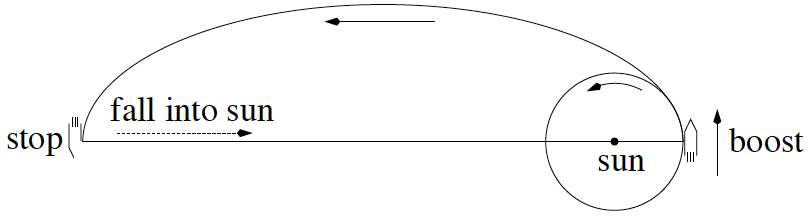
\includegraphics[scale=0.6]{Graphics/h8p1}
\end{center}

(c) Calculate the impulse $I_1$ required at the first rocket burn (the boost). Express your answer in terms of $I_0$, $R$ and $r$.''

Okay, so aphelion is the furthest it ever comes from the Sun (perihelion is the closest). If we call aphelion point A, perihelion point P and the Sun point Q, then we have AQ + PQ = $2a$, where $a$ is the orbit's semi-major axis.\\
If the distance AQ is $r$, and the current distance PQ from us to the Sun is $R$, then via the diagram provided, clearly $2a = R + r$, where $a$ is the semi-major axis of the new, elliptical orbit.

Combined with the next question, we need to find the impulse required to move into an elliptical orbit with new speed $v_1$, such that $\displaystyle a = \frac{R + r}{2}$.

We make a burn so that the new speed is $v_1$, and the new (linear) momentum $m v_1$. The impulse is then $m(v_1 - v_0)$, but we don't know $v_1$ yet.\\
We can figure out $v_1$ by conservation of energy. \emph{After} the burn, energy is conserved (but not during, of course). The new kinetic energy, plus the new (same as before) potential energy must equal half of the potential energy of the new, elliptical orbit:

\begin{align}
\frac{1}{2} m v_1^2 - \frac{m M G}{R} = -\frac{m M G}{2a}
v_1^2 &= \frac{2 M G}{R} - \frac{M G}{a}\\
v_1^2 &= 2 M G\left(\frac{1}{R} - \frac{1}{2a}\right)\\
v_1   &= \sqrt{2 M G\left(\frac{1}{R} - \frac{1}{R + r}\right)} = \sqrt{\frac{2 G M r}{R(R + r)}}
\end{align}

Now, here's the slightly tricky part... We know that $\displaystyle v_0 = \sqrt{\frac{M G}{R}}$, and we need to write the above in terms of $v_0$. Thankfully, with the simplification done, that is in fact now the opposite of tricky. It could have been! We simply remove those variables from inside the square root, and tack on $v_0$ outside:

\begin{equation}
v_1 = v_0 \sqrt{\frac{2 r}{(R + r)}}
\end{equation}

Next, we need to write this in terms of impulse. $I_0 = v_0/m$, and $I_1 = m(v_1 - v_0)$.

\begin{align}
I_1 = m v_0 \sqrt{\frac{2 r}{(R + r)}} - m v_0 = I_0 \left(\sqrt{\frac{2 r}{(R + r)}} - 1\right)
\end{align}

``(d) What is the speed $v_2$ of the spacecraft at aphelion? Express your answer in terms of $v_0$, $R$ and $r$.''

Finally, we need to convert $v_1$ into $v_2$. $v_1$ at perihelion, and $v_2$ is at aphelion. The speed at perihelion is much greater than that at aphelion.\\
Angular momentum is the same at both locations. Therefore, $R m v_1 = r m v_2$, or $R v_1 = r v_2 \Rightarrow v_2 = \frac{R}{r} v_1$.

\begin{equation}
v_2 = \frac{R}{r} v_0 \sqrt{\frac{2r}{R + r}}
\end{equation}

``(e) Calculate the impulse $I_2$ required at the second rocket burn (at aphelion). Express your answer in terms of $I_0$, $R$ and $r$.''

This shouldn't be too bad now. We need to bring $v_2$ down to zero, so

\begin{equation}
I_2 = m v_2 = m v_0 \frac{R}{r} \sqrt{\frac{2r}{R + r}} = I_0 \frac{R}{r} \sqrt{\frac{2r}{R + r}}
\end{equation}

Again, they want a positive value.

``(f) Compare the impulse under b) with the sum of the impulses under c) and e) (i.e find $I_0 - (I_1 + I_2)$), and convince yourself that the latter procedure is more economical. Express your answer in terms of $I_0$, $R$ and $r$.''

I will call this $\Delta I$ for a lack of a better name.

\begin{align}
\Delta I &= I_0 - \left( I_0 \left(\sqrt{\frac{2 r}{(R + r)}} - 1\right) + I_0 \frac{R}{r} \sqrt{\frac{2r}{R + r}} \right)\\
\Delta I &= I_0 - I_0 \left( \sqrt{\frac{2 r}{(R + r)}} - 1 + \frac{R}{r} \sqrt{\frac{2r}{R + r}} \right)
\end{align}

To convince ourselves, we need to find that the expression in parenthesis is always such that $\Delta I > 0$ (otherwise, it's equally or even less efficient).

\begin{align}
\Delta I &= I_0 - I_0 \left( \sqrt{\frac{2 r}{(R + r)}} \left(1 + \frac{R}{r}\right) - 1 \right)\\
\Delta I &= 2 I_0 - I_0 \left( \sqrt{\frac{2 r}{(R + r)}} \left(1 + \frac{R}{r}\right) \right)\\
\Delta I &= I_0\left( 2 - \sqrt{2} \sqrt{\frac{R+r}{r}} \right)
\end{align}

Finally, we can truly convince ourselves by solving this for $r$ manually:

\begin{align}
2 - \sqrt{2} \sqrt{\frac{R+r}{r}} &> 0\\
\sqrt{2} \sqrt{\frac{R+r}{r}} &< 2\\
2 \frac{R+r}{r} &< 4\\
2 R &< 2r\\
R &< r
\end{align}

So indeed, for \emph{any} chosen $r > R$, this is more efficient. Of course, we need to remain in orbit for the result to be useful; we could of course make a ridiculous burn to reach an extremely high speed and escape, which would be less efficient, but in that case, we would have any $r$ as we would not be in an elliptical orbit.

Phew! This took a very long time for me -- a while to figure out how to solve part (c), and a \emph{very} long time to figure out where I was going wrong. I got $v_0$ correct at once, but then accidentally wrote down an incorrect expression in my notes: $\displaystyle v_0 = \sqrt{\frac{2 M G}{R}}$. You may notice that is the escape velocity for Earth's orbit, not $v_0$ -- I did too, only the day after I started working on this problem. Once I noticed, everything else went rather smoothly.

\section{Problem 2: Black hole in X-ray binary}

``An X-ray binary consists of 2 stars with masses $m_1$ (the accreting compact object) and $m_2$ (the donor). The orbits are circular with radii $r_1$ and $r_2$ centered on the center of mass.

\begin{center}
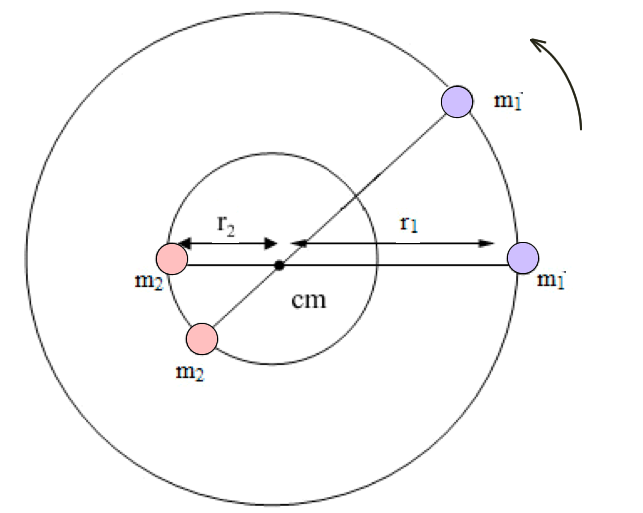
\includegraphics[scale=0.5]{Graphics/h8p2}
\end{center}

(a) Find the orbital period $T$ of the binary following the guidelines given in lectures. Express your answer in terms of $(m_1+m_2)$, $(r_1+r_2)$ and $G$.\\
(b) In the case of Cyg X-1 (as discussed in lectures), the orbital period is 5.6 days. The donor star is a ``supergiant'' with a mass 30 times that of the sun. Doppler shift measurements indicate that the donor star has an orbital speed $v_2$ of about 148 km/sec. Calculate $r_2$ (in meters).\\
(c) Calculate $r_1$ (in meters).\\
(d) Now calculate the mass m1 of the accreting compact object (express that as ratio to the mass of the sun $m_1/M_{Sun}$).''

Well, part (a) is easy, at least. We even saw that expression, exactly as-is, during the lecture (indeed, in the part about Cygnus X-1, i.e. this system).\\
We use the equation for periods of elliptical orbits, sometimes known as Kepler's third law (though Kepler only said $T^2 \propto a^3$; the rest was calculated later), only we substitute in $m_1 + m_2$ for the mass, and $r_1 + r_2$ for the orbital radius:

\begin{equation}
T = \sqrt{\frac{4 \pi^2 (r_1 + r_2)^3}{G (m_1 + m_2)}}
\end{equation}

For part (b), they tell us the period $T$, and the velocity $v_2$. Finding $r_2$ is a piece of cake, then, if we don't get wrapped up in complex thinking!

\begin{equation}
\frac{2 \pi r_2}{T} = v_2
\end{equation}

\begin{equation}
r_2 = \frac{v_2 T}{2 \pi} = \frac{(\SI{148e3}{m/s})(\SI{5.6}{days})}{2 \pi} \approx \SI{1.1397e10}{m}
\end{equation}

We now know $T$ and $r_2$, but not $m_1$, $m_2$ or $r_1$. For finding $r_1$, they gave us a hint, though:

``Hint: Your calculations will be greatly simplified if instead of $r_1$ you set up your equations in terms of $r_1/r_2$, and using some relation between the distances and the masses. Once you express your equation in terms of $r_1/r_2$, you will find a third order equation in $r_1/r_2$. Only one solution is real; the other two are imaginary. There are various ways to find an approximation for $r_1/r_2$. You can find the solution by trial and error using your calculator, or you can plot the function.''

Hmm. Well, via the center of mass definition,

\begin{equation}
m_1 r_1 = m_2 r_2
\end{equation}

We can certainly find $r_1/r_2$ from that:

\begin{equation}
\frac{r_1}{r_2} = \frac{m_2}{m_1}
\end{equation}

They also tell us that $m_2 = 30 M_{Sun}$.

\begin{equation}
r_1 = \frac{30 M_{Sun}}{m_1} r_2
\end{equation}

Here is where we need to start applying the hint given. I will copy the staff solution a bit here (i.e. I'm writing this part after the deadline has passed to clean up). We can assign a variable $x = r_1/r_2$.\\
This then implies that $m_1 = m_2/x$ using the above relationships.

We can now start rewriting the period equation. First, we square it to get rid of the square root on the right-hand side. Then, we factor out $r_2^3$ and $m_2$, respectively, out of the parenthesis, to get the insides in fraction form:

\begin{equation}
T^2 = \frac{4 \pi^2 r_2^3(\frac{r_1}{r_2} + 1)^3}{G m_2 (\frac{m_1}{m_2} + 1)}
\end{equation}

Next, we write this in terms of $x$:

\begin{equation}
T^2 = \frac{4 \pi^2 r_2^3(x + 1)^3}{G m_2 (\frac{1}{x} + 1)}
\end{equation}

Finally, we isolate $x$ on the right hand side:

\begin{equation}
\frac{G m_2 T^2}{4 \pi^2 r_2^3} = \frac{(x + 1)^3}{\frac{1}{x} + 1}
\end{equation}

We can now approximate this function. We know everything on the left-hand side: $m_2 = 30 M_{Sun} = 30 \times \SI{2e30}{kg}$, $T = 5.6$ days times 86400 seconds and $r_2 = \SI{1.1397e10}{m}$.\\
The left-hand side is approximately equal to $16.04$.

We can then plot the two functions

\begin{align}
y &= 16.04\\
y &= \frac{(x + 1)^3}{\frac{1}{x} + 1}
\end{align}

and see where they intersect. That happens at approximately $x = 1.9031$.

With that value in hand, we can now find $r_1 = x r_2 = \SI{2.169e10}{m}$ and $m_1 = m_2/x = 15.764$ solar masses.

\section{Problem 3: Torque, rotation and translation}

``A Yo-Yo of mass m has an axle of radius $b$ and a spool of radius $R$. Its moment of inertia about the center can be taken to be $\displaystyle I = \frac{1}{2}m R^2$ and the thickness of the string can be neglected. The Yo-Yo is released from rest. You will need to assume that the center of mass of the Yo-Yo descends vertically, and that the string is vertical as it unwinds.

\begin{center}
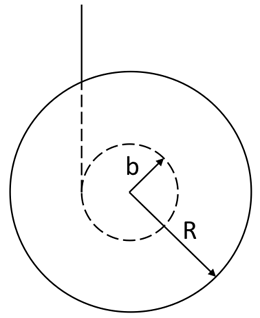
\includegraphics[scale=0.45]{Graphics/h8p3}
\end{center}

(a) What is magnitude of the tension in the cord as the Yo-Yo descends? Express your answer in terms of $m$, $b$, $R$ and acceleration due to gravity $g$.\\
(b) Find the angular speed of the Yo-Yo when it reaches the bottom of the string, when a length $\ell$ of the string has unwound. Express your answer in terms of $m$, $b$, $R$, $\ell$ and acceleration due to gravity $g$.\\
(c) Find the magnitude of the average tension in the string over the course of the Yo-Yo reversing its direction at the bottom of its descent (see figure below). Express your answer in terms of $m$, $b$, $R$, $\ell$ and acceleration due to gravity $g$.''

\begin{center}
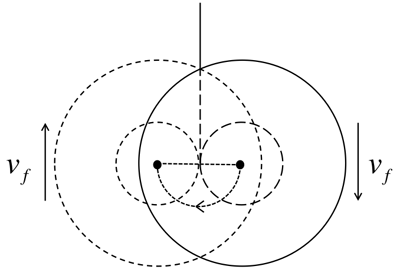
\includegraphics[scale=0.5]{Graphics/h8p3_2}
\end{center}

Let's see. First, we can write an equation for the acceleration of the center of mass, in terms of string tension acting upwards, and gravity acting downwards. We choose downwards to be the positive direction, and find

\begin{equation}
m a = m g - T
\end{equation}

Next, we can consider the torque. I will do so considering the center of the yo-yo, call it point C:

\begin{equation}
\tau_C = I_C \alpha
\end{equation}

The torque is due to the tension acting on the inner spool of radius $b$, and is $\tau_C = T b$.\\
We can also use the relationship $a = \alpha R$, which holds if there is no slipping. With these two things in mind, we can rewrite the above equation as

\begin{equation}
T b = I_C \frac{a}{b}
\end{equation}

We can solve for the tension by solving these for A and setting them equal.

\begin{align}
a &= g - \frac{T}{m}\\
a &= \frac{T b^2}{I_C}
\end{align}

\begin{align}
g - \frac{T}{m} &= \frac{T b^2}{I_C}\\
g &= T\left(\frac{b^2}{I_C} + \frac{1}{m}\right)\\
\frac{g}{\frac{b^2}{I_C} + \frac{1}{m}} &= T
\end{align}

We are given that $I_C = \frac{1}{2} m R^2$, so we can stick that in there and simplify to find the tension in terms of the variables they want:

\begin{align}
\frac{g}{\frac{b^2}{(1/2) m R^2} + \frac{1}{m}} &= T\\
\frac{m g}{2 \frac{b^2}{R^2} + 1} &= T\\
\frac{m g R^2}{2 b^2 + R^2} &= T
\end{align}

Next, they want the angular speed when the Yo-Yo reaches the bottom.\\
Now, we have a situation equivalent to pure roll, which means that the tangential velocity is always equal to the velocity of the center of mass.\\
We can therefore solve this more easily (I believe it's easier, anyway) by using $a$, using that to find the velocity of the center of mass, which then is equal to the tangential velocity, and converting that to angular speed.

We have an expression for the acceleration as a function of $T$, and we know $T$, so

\begin{equation}
a = g \left(1 - \frac{R^2}{2 b^2 + R^2}\right)
\end{equation}

Since the acceleration is clearly constant in time, the velocity as a function of acceleration is just $v = a t$, but we don't know $t$.\\
We can use a second constant acceleration kinematics equation, though: $\ell = \frac{1}{2} a t^2$. We solve that one for $t$:

\begin{align}
\ell &= \frac{1}{2} a t^2\\
\sqrt{\frac{2 \ell}{a}} &= t
\end{align}

Combining the two,

\begin{equation}
v_f = a \sqrt{\frac{2 \ell}{a}} = \sqrt{2 \ell a} = \sqrt{2 \ell} \sqrt{g \left(1 - \frac{R^2}{2 b^2 + R^2}\right)}
\end{equation}

Finally, to convert to angular speed, we simply use $v_f = \omega b$, so $\omega = \frac{v_f}{b}$:

\begin{equation}
\omega = \frac{\sqrt{2 \ell}}{b} \sqrt{g \left(1 - \frac{R^2}{2 b^2 + R^2}\right)}
\end{equation}

This can be simplified quite a bit further (I used Mathematica for this one):

\begin{equation}
\omega = 2 \sqrt{\frac{g \ell}{2 b^2 + R^2}}
\end{equation}

We should be able to solve the last part in terms of impulse. If the speed $v_f$ going back up is the same as the speed down, as the diagram shows, the impulse is $2 m v_f$.\\
The average force acting on the yo-yo is found via

\begin{equation}
I = \Braket{F} \Delta t
\end{equation}

However, the average force and the average tension are not the same thing. Regardless of the tension, there is clearly a constant downwards force $m g$ acting on the yo-yo, due to gravity. Let's take care of that last.

\begin{equation}
\frac{2 m v_f}{\Delta t} = \Braket{F}
\end{equation}

Of course, this causes a new problem: what is $\Delta t$? We know the speed $v_f$ just prior to and just after, but what about during this turnaround?\\
Because the angular velocity is about the same for the entire turnaround (it doesn't switch directions), $v_f$ is also approximately constant, since the two are linearly proportional.

In that case, $\Delta t = d/v_f$, where $d$ is the distance traveled during this time. So what is \emph{that}, then? I would think it is half the circumference of the inner spool, which is $\pi b$. We can then find the time as the distance divided by the tangential velocity, $\Delta t = (\pi b)/v_f$, so using that, plus our expression of the velocity $v_f$ as the string is unwrapped:

\begin{align}
\frac{2 m v_f^2}{\pi b} &= \Braket{F}\\
\frac{2 m}{\pi b} 2 \ell g \left(1 - \frac{R^2}{2 b^2 + R^2}\right) &= \Braket{F}
\end{align}

(Side note added afterwards: we can just as easily, probably more easily, consider that it moves $\pi$ radians about the inner spool, and use $\omega$ at the turnaround point to calculate the time taken.)

Let's now not forget that $\Braket{F}$ is the average \emph{net} force on the object. Gravity is pulling it down, which the tension is trying to counteract. Therefore, we \emph{add} $m g$, $\Braket{F_{gravity}}$ (which is thankfully a constant) to the above to find the average tension:

\begin{align}
m g + \frac{2 m}{\pi b} 2 \ell g \left(1 - \frac{R^2}{2 b^2 + R^2}\right) &= \Braket{T_r}\\
m g + \frac{4 m \ell g}{\pi b} \left(1 - \frac{R^2}{2 b^2 + R^2}\right) &= \Braket{T_r}
\end{align}

Again, this can be simplified quite a bit, and again, I used Mathematica for that part:

\begin{equation}
\Braket{T_r} = m g \left(\frac{8 b \ell}{2 \pi b^2 + \pi R^2} + 1\right) + m 
\end{equation}

\section{Problem 4: Double block pulley}

``A pulley of mass $m_p$, radius $R$, and moment of inertia about its center of mass $I_c$, is attached to the edge of a table. An inextensible string of negligible mass is wrapped around the pulley and attached on one end to block 1 that hangs over the edge of the table. The other end of the string is attached to block 2 which slides along a table. The coefficient of sliding friction between the table and the block 2 is $\mu_k$ . Block 1 has mass $m_1$ and block 2 has mass $m_2$, with $m_1 > \mu_k m_2$. At time $t = 0$, the blocks are released from rest. At time $t = t_1$, block 1 hits the ground. Let $g$ denote the gravitational acceleration near the surface of the earth.

\begin{center}
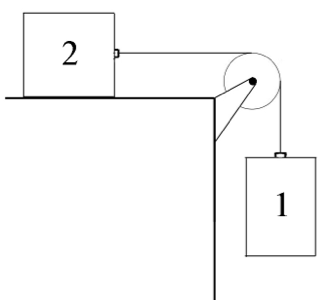
\includegraphics[scale=1.1]{Graphics/h8p4}
\end{center}

(a) Find the magnitude of the linear acceleration of the blocks. Express your answer in terms of $m_1$, $m_2$, $I_c$, $R$, $\mu_k$ and $g$ as needed.\\
(b) How far did the block 1 fall before hitting the ground? Express your answer in terms of $m_1$, $m_2$, $I_c$, $R$, $\mu_k$, $t_1$ and $g$ as needed.''

All right, time to look at some forces, to begin with!\\

Block 2 has four forces acting on it: $m g$ downwards, $N = m g$ upwards (since there is no acceleration along the $y$ axis, they must cancel), a tension $T_2$ towards the right, and friction $F_f = \mu_k m_2 g$ towards the left.\\
Block 1 has only two: $m g$ downwards, and $T_1$ upwards.

Newton's second law for the two gives us, taking downwards (block 1) = rightwards (block 2) as positive:
\begin{align}
m_2 a &= T_2 - \mu_k m_2 g\\
m_1 a &= m_1 g - T_1
\end{align}

Next, we can consider the torque and angular acceleration of the pulley. Relative to the center C of the pulley, the torque is $I_c \alpha$. As usual, we use $a = \alpha R$ to rewrite this in terms of the linear acceleration $a$, and assume there is no slipping or such going on.

\begin{equation}
\tau_C = I_c \frac{a}{R}
\end{equation}

So what is the torque? Well, we can write it as the torque due to $T_1$ (which causes clockwise rotation) minus the torque due to $T_2$. Both act at 90 degree angles with the center, so

\begin{equation}
R (T_1 - T_2) = I_c \frac{a}{R}
\end{equation}

We now have three equations and three unknowns: $a$, $T_1$ and $T_2$.
If we solve the tension equations for $T_2$ and $T_1$ respectively, we can find $T_1 - T_2$ easily, and therefore $a$.\\
First, I will solve the above equation for $a$:

\begin{equation}
a = \frac{R^2}{I_c} (T_1 - T_2)
\end{equation}

Solving the two is also easy:

\begin{align}
m_2 a + \mu_k m_2 g &= T_2\\
m_1 g - m_1 a &= T_1
\end{align}

All that remains is to combine the three as mentioned, and solve for $a$:

\begin{align}
a &= \frac{R^2}{I_c} (m_1 g - m_1 a - m_2 a - \mu_k m_2 g)\\
a &= \frac{R^2}{I_c} (m_1 g - \mu_k m_2 g) - \frac{R^2}{I_c} m_1 a - \frac{R^2}{I_c} m_2 a\\
a \left(1 +\frac{R^2 m_1}{I_c} + \frac{R^2 m_2}{I_c}\right) &= \frac{R^2}{I_c} (m_1 g - \mu_k m_2 g)\\
a &= \frac{\frac{R^2}{I_c} (m_1 g - \mu_k m_2 g)}{1 +\frac{R^2 m_1}{I_c} + \frac{R^2 m_2}{I_c}}\\
a &= \frac{g R^2 (m_1 - \mu_k m_2)}{I_c + R^2 (m_1 + m_2)}
\end{align}

Well then! Let's see about part (b).\\
Is the acceleration constant? Yes, it is; nothing in there should change over time. Therefore, we can answer this one using some very basic kinematics:

\begin{equation}
d = \frac{1}{2} a t_1^2 = \frac{1}{2} \frac{g R^2 (m_1 - \mu_k m_2)}{I_c + R^2 (m_1 + m_2)} t_1^2
\end{equation}

\section{Problem 5: Wheel, inclined plane, two masses and a rope}

``A wheel in the shape of a uniform disk of radius $R$ and mass $m_p$ is mounted on a frictionless horizontal axis. The wheel has moment of inertia about the center of mass $\displaystyle I_{cm} = \frac{1}{2} m_p R^2$. A massless cord is wrapped around the wheel and one end of the cord is attached to an object of mass $m_2$ that can slide up or down a frictionless inclined plane. The other end of the cord is attached to a second object of mass $m_1$ that hangs over the edge of the inclined plane. The plane is inclined from the horizontal by an angle $\theta$. Once the objects are released from rest, the cord moves without slipping around the disk. Find the magnitude of accelerations of each object, and the magnitude of tensions in the string on either side of the pulley. Assume that the cord doesn't stretch ($a_1 = a_2 = a$). Express your answers in terms of the masses $m_1$, $m_2$, $m_p$, angle $\theta$ and the gravitational acceleration due to gravity near earth's surface $g$.''

\begin{center}
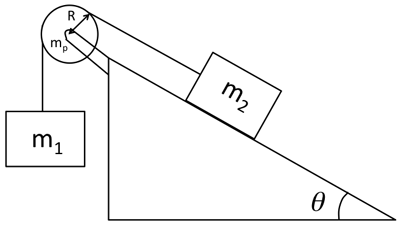
\includegraphics[scale=0.5]{Graphics/h8p5}
\end{center}

They then ask for $a$, $T_1$ (tension at $m_1$) and $T_2$ (tension at $m_2$).\\
This certainly looks like the slightly more complex brother of the previous problem!

To begin with, we can't know which of the masses will ``win'', if any. If static friction wins, then $a = 0$, which is the trivial solution and one that I will not even attempt to submit. What happens otherwise? Well, getting the sign correct is guesswork, as far as I can tell; according to forum discussions, this seems to be the consensus. I will call downwards (for $m_1$) and uphill (for $m_2$) positive in this solution.

Well then! We yet again have a bunch of forces. The forces on the hanging mass are unchanged, so we get the same equation there:

\begin{equation}
m_1 a = m_1 g - T_1
\end{equation}

Block 2 changes the game a little. We have the same four forces, but we now need to decompose the gravitational force into the normal force component and the ``downhill'' component.
Performing the decomposition, we find the normal force as $m_2 g \cos \theta$, which the downhill force is $m_2 g \sin \theta$.\\
The incline is frictionless, so gravity is the only downhill force. There is a tension $T_2$ uphill, however, All in all, the normal force cancels out the component of gravity perpendicular to the incline, while $T_2$ uphill and $m_2 g \sin \theta$ battles where the block should move.\\
Using the directions I chose,

\begin{equation}
m_2 a = T_2 - m_2 g \sin \theta
\end{equation}

Two equations, three unknowns. We need to consider the pulley next, as usual in these problems.\\
As in the previous problem, the tensions cause a torque, and both are perpendicular to the center of the wheel. The torque relative to the pulley's center is $\tau_C = R(T_1 - T_2)$, which again is equal to $I_{cm} \alpha = I_{cm} \frac{a}{R}$. We were given $I_{cm}$ in terms of mass and radius:

\begin{align}
R(T_1 - T_2) &= \frac{1}{2} m_p R a\\
\frac{2(T_1 - T_2)}{m_p} &= a
\end{align}

I will again find $T_1 - T_2$ by solving those two equations individually and subtracting them:

\begin{align}
m_1 g - m_1 a &= T_1\\
m_2 a + m_2 g \sin \theta &= T_2
\end{align}

\begin{equation}
T_1 - T_2 = m_1 g - m_1 a - m_2 a - m_2 g \sin \theta
\end{equation}

Substitute that in to the torque equation:

\begin{align}
a &= \frac{2}{m_p} \left(m_1 g - m_1 a - m_2 a - m_2 g \sin \theta \right)\\
a &= \frac{2}{m_p} \left(m_1 g - m_2 g \sin \theta \right) - \frac{2 m_1}{m_p} a - \frac{2 m_2}{m_p} a\\
a \left(1 + \frac{2 m_1}{m_p} + \frac{2 m_2}{m_p}\right) &= \frac{2}{m_p} \left( m_1 g - m_2 g \sin \theta \right)\\
a &= \frac{\frac{2}{m_p} \left(m_1 g - m_2 g \sin \theta \right)}{1 + \frac{2 m_1}{m_p} + \frac{2 m_2}{m_p}}\\
a &= \frac{2 g \left(m_1 - m_2 \sin \theta \right)}{m_p + 2 m_1 + 2 m_2}\\
\end{align}

We can then find the tensions easily, since we solved for them earlier. Whether it will be pretty is a different matter!

\begin{equation}
T_1 = m_1 \left( g - \frac{2 g \left(m_1 - m_2 \sin \theta \right)}{m_p + 2 m_1 + 2 m_2} \right)
\end{equation}

\begin{equation}
T_2 = m_2 \left(g \sin \theta + \frac{2 g \left(m_1 - m_2 \sin \theta \right)}{m_p + 2 m_1 + 2 m_2} \right)
\end{equation}

\section{Problem 6: Rolling object on an incline}

``A hollow cylinder of outer radius $R$ and mass $M$ with moment of inertia about the center of mass $I_{cm} = M R^2$ starts from rest and moves down an incline tilted at an angle $\theta$ from the horizontal. The center of mass of the cylinder has dropped a vertical distance $h$ when it reaches the bottom of the incline. Let $g$ denote the acceleration due to gravity. The coefficient of static friction between the cylinder and the surface is $\mu_s$. The cylinder rolls without slipping down the incline. The goal of this problem is to find an expression for the smallest possible value of $\mu_s$ such that the cylinder rolls without slipping down the incline plane and the velocity of the center of mass of the cylinder when it reaches the bottom of the incline.

\begin{center}
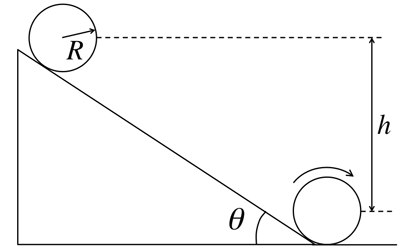
\includegraphics[scale=0.5]{Graphics/h8p6}
\end{center}

(a) What is the magnitude of the acceleration $a$ of the center of mass of the cylinder on the incline? Express your answer in terms of $\theta$ and $g$ as needed.\\
(b) What is the minimum value for the coefficient of static friction $\mu_s$ such that the cylinder rolls without slipping down the incline plane? Express your answer in terms of $\theta$.\\
(c) What is the magnitude of the velocity of the center of mass of the cylinder when it reaches the bottom of the incline? Express your answer in terms of $g$ and $h$ as needed.''

Okay, so let's see. First, what happens with zero friction? Clearly, there is no rolling at all, since there will be no torque on the cylinder.\\
For there to be pure roll, a condition that must be fulfilled is that the tangential speed $\omega R$ is the same as the velocity at the center of mass. Since the angular acceleration is $\alpha = a/R$, we must have $\alpha R = a$ for pure roll to hold.

Let's start out with part (a) and see where that leads.\\
If there is is no slipping, then there is no kinetic friction. There is, however, \emph{static} friction. Without that, the cylinder would slide down without turning at all.

If we choose a coordinate system where $y$ is perpendicular to the incline, while $x$ is downhill, we can write the the normal component of gravity as $M g \cos \theta$, while the downhill component is $M g \sin \theta$. Static friction acts upwards: the friction must be such that the torque causes clockwise rotation (or it would roll the wrong way!). This implies an uphill frictional force, $\mu_s N = \mu_s M g \cos \theta$. (Another way to think of it is that the cylinder wants to slide downhill. Therefore, static friction acts uphill, since friction always \emph{opposes} relative motion between surfaces.) 

\begin{align}
M a &= M g \sin \theta - \mu_s M g \cos \theta\\
a &= g (\sin \theta - \mu_s \cos \theta)
\end{align}

This would seem to answer part (a), but we're not allowed to use $\mu_s$ in the answer, so we need to keep working.

As mentioned earlier, in this analysis, the cylinder rolls due to the torque caused by friction. Friction acts uphill, and the magnitude of the torque, relative to the center of the cylinder, is $R F_f = R M g \mu_s \cos \theta$.

A useful relation is then that $\displaystyle \tau = I_{cm} \alpha = I_{cm} \frac{a}{R}$ (the latter part holds for pure roll only), and we are given that $I_{cm} = M R^2$, so

\begin{align}
R M g \mu_s \cos \theta &= a M R
\end{align}

$M$ and $R$ both cancel.\\
We can solve this for $\mu_s$:

\begin{align}
g \mu_s \cos \theta &= a\\
\mu_s &= \frac{a}{g \cos \theta}
\end{align}

This gives us the acceleration, now that we can write $\mu_s$ in terms of $g$ and $\cos \theta$:

\begin{align}
a &= g (\sin \theta - \frac{a}{g \cos \theta} \cos \theta)\\
a &= g \sin \theta - a\\
a &= \frac{g \sin \theta}{2}
\end{align}

Next, we substitute this back into $\mu_s$ to get it in terms of $\theta$:

\begin{align}
\mu_s &= \frac{\frac{g \sin \theta}{2}}{g \cos \theta}\\
\mu_s &= \frac{\tan \theta}{2}
\end{align}

Very nice and simple! This is the \emph{minimum} amount of friction required for pure roll. More friction wouldn't hurt; as the acceleration equation shows, more friction doesn't cause less acceleration, but it does prevent sliding.

Finally, what is the velocity of the center of mass as it reaches the bottom? Well, we know the acceleration. We could use the work-energy theorem, but there will be both linear kinetic energy and rotational kinetic energy, so that seems like it would be harder. Then again, we don't know the \emph{time} which we need for kinematics, so I will go the energy route anyway.\\
The final velocity $v$ causes an angular velocity $v = \omega/R$ with no sliding. The total kinetic energy can be written down as being equal to $M g h$, which is the total energy available to be converted:

\begin{align}
K_{lin} + K_{rot} &= M g h\\
\frac{1}{2} M v^2 + \frac{1}{2} I_{cm} \omega^2 &= M g h\\
\frac{1}{2} M v^2 + \frac{1}{2} (M R^2) \left(\frac{v}{R}\right)^2 &= M g h\\
\frac{1}{2} M v^2 + \frac{1}{2} M v^2 &= M g h\\
v^2 &= g h\\
v &= \sqrt{g h}
\end{align}

Nice! The intermediate results were semi-complex at times, but the answers are all dead simple.

There are several interesting things in this result, at least two of which I didn't realize until a few days after solving this. One is that the rotational kinetic energy in this case is exactly equal to the linear kinetic energy -- the expression on the right in equation 4 above simplifies to $\frac{1}{2} M v^2$!\\
Without this term, the velocity would be $\sqrt{2 g h}$ instead, i.e. exactly a factor $\sqrt{2}$ greater, regardless of much of anything else.\\
(I rewrote that equation after realizing this; I previously had it in a form which made this hard to see.)

Second, I chose to analyze this relative to the center, which means that static friction provides a torque. How can there be an increase in rotational kinetic energy without a torque that does positive work? As far as I know, there certainly cannot. Therefore, according to this analysis, static friction provides this positive work!\\
\emph{However}, it still does no net work, which is the amazing thing: it is a linear force uphill, which therefore fights with $M g \sin \theta$ about the linear acceleration. It therefore acts to reduce the final linear velocity by a factor $1/\sqrt{2}$, and the final kinetic energy by a factor $1/2$; this is instead turned into rotational kinetic energy here.

So while static friction appears to does positive work increasing the rotational kinetic energy, it appears to do an equal amount of negative work in the linear motion, for a net of zero work -- as it must be.

If we instead analyze this problem relative to the point of contact, friction can provide no torque (as it acts through that point), and we will instead find gravity providing the torque and therefore doing the work that gets the cylinder rolling. For other points, where both forces can cause a torque relative to the center, we should find some combination of the two effects, but with the same end result.

\section{Problem 7: Space debris collision}

``A satellite of mass $m$ is orbiting the earth, mass $M$, in a circular orbit of radius $r_a$. Unfortunately a piece of space debris left by a passing rocket lies directly in the satellite's path. The piece of debris has the same mass $m$ as the satellite. The debris collides with the satellite and sticks to the satellite. Assume that the debris has negligible speed just before the collision. After the collision, the satellite and debris enter an elliptical orbit around the earth. The distance of closest approach to the earth of the satellite and the debris is $r_p$. Let $G$ be the universal constant of gravity. You may assume that $M \gg m$.

\begin{center}
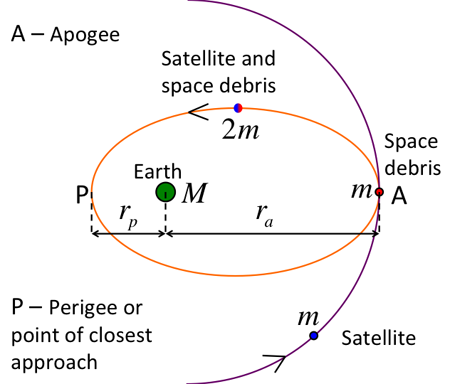
\includegraphics[scale=0.65]{Graphics/h8p7}
\end{center}

(a) Find an expression for the speed $v_0$ of the satellite before the collision. You may express your answer in terms of $M$, $r_a$ and $G$ as needed.\\
(b) Calculate the ratio $r_a/r_p$.''

I wonder how realistic the answers will be -- a piece of debris with negligible speed (relative to the Earth) wouldn't stay in place for very long!

The satellite begins with linear momentum $m v_0$. After the hit, the mass doubles, and so velocity is cut in half. Call this post-hit velocity $v_a$ (a for apogee); using conservation of (linear) momentum, we then have $m v_0 + 0 = 2m v_a$, so indeed $\displaystyle v_a = \frac{v_0}{2}$.\\
We could also find this relationship using conservation of angular momentum relative to the center of the Earth, by the way.

Given this ``initial'' velocity $v_a$ and the initial distance to the Earth, we could find the orbital parameters for the new elliptical orbit, but I don't believe we will need all of them. Clearly, the apogee distance $r_a$ is simply the initial radius of the circular orbit, which is even given in the problem, only they don't mention it explicitly, but use the same variable for the two (and draw the graphic showing the two are equal).

Now, then. How can we calculate $v_0$? Well, we know the orbital radius, and for a circular orbit, each orbital radius has  unique velocity. This velocity can be derived by remembering that the total mechanical energy is always $\frac{1}{2} U$, but I'm confident that I remember the quite simple velocity equation, so:

\begin{equation}
v_0 = \sqrt{\frac{M G}{r_a}}
\end{equation}

$r_a + r_p = 2 a$, where $a$ is the elliptical orbit's semi-major axis. Via an energy calculation, we can relate the new velocity $v_a$ plus the current potential energy with the total mechanical energy for an elliptical orbit, which depends on $2a$, so we can find $a$.

\begin{align}
\frac{1}{2} (2m) v_a^2 - \frac{2m M G}{r_a} = - \frac{2m M G}{2a}\\
v_a^2 - \frac{2 M G}{r_a} = - \frac{2 M G}{2a}\\
\frac{1}{v_a^2 - \frac{2 M G}{r_a}} = - \frac{a}{M G}\\
\frac{M G}{\frac{2 M G}{r_a} - v_a^2} = a\\
\frac{r_a M G}{2 M G - r_a v_a^2} = a
\end{align}

Since we know that $r_a + r_p = 2a$, the above must be equal to $\frac{r_a+r_p}{2}$. We can also substitute in the value for $v_a = v_0/2 = \frac{1}{2} \sqrt{\frac{M G}{r_a}}$:

\begin{align}
\frac{r_a M G}{2 M G - r_a \frac{M G}{4 r_a}} = \frac{r_a + r_p}{2}\\
\frac{4 r_a M G}{8 M G - M G} = \frac{r_a + r_p}{2}\\
\frac{8 r_a}{7} - r_a = r_p\\
\frac{r_a}{7} = r_p
\end{align}

Well, that sure became simple. The ratio is then $r_a/r_p = 7$ -- showing that the apogee is at a (much) greater than distance than the perigee, as one would expect.

And that's it for this problem!

\section{Problem 8: Turntable solutions}

\begin{center}
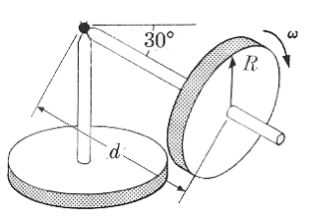
\includegraphics[scale=1.2]{Graphics/h8p8}
\end{center}

``A gyroscope consists of a uniform disc of mass radius $M = 2$ kg and radius $R = 0.3$ m. The disc spins with an angular speed $\omega = 400$ rad/s as shown in the figure [above]. The gyroscope precesses, with its axle at an angle $\ang{30}$ below the horizontal (see figure). The gyroscope is pivoted about a point $d = 0.6$ m from the center of the disc. What is the magnitude of the precessional angular velocity $\Omega$ (in radians/sec)?''

Time for a short break to read the textbook! I'm unsure whether we can use $\displaystyle \Omega = \frac{\tau}{I_c \omega}$ here (after vector decomposition), or not.\\
They indeed seem to consider that we can ignore any angular momentum due to the orbital motion, and therefore, this approximation should be valid. Very well, then.\\
My solution will be less rigorous than the quite technical discussion in the textbook; if you want more detail, I recommend having a look there. Actually, I would recommend that either way!

The torque relative to what I will call point P, the pivot point where the axle meets the stand, is $\tau_P = \vec{d} \times \vec{F_{gr}} = (\vec{d} \times \vec{g})M$. Unlike what we have seen previously, the angle is not 90 degrees. Gravity is always straight downwards, of course, but as the angle the axle makes with the horizontal grows (downwards), the torque goes down. It is at a maximum with $\theta = 0$, and zero when the axle is pointing straight down (which makes sense: the two vectors are then anti-parallel, so the cross product must be zero). The equation then becomes

\begin{equation}
\tau_p = \vec{d} \times \vec{F_g} = d M g \cos \theta
\end{equation}

(where $\theta$ is the angle that is marked as 30 degrees).

Why a cosine, in a cross product? Because the angle \emph{between the two vectors} is not equal to the $\ang{30}$ degrees shown, but instead is $\ang{90} - \ang{30}$ degrees. It makes intuitive sense that when the angle shown is zero, the torque is at a maximum, and when the axle is vertical, there is zero torque.\\
We could write the cross product as $d M G \sin \alpha$, where $\alpha$ is the angle between the vectors, followed by $\alpha + \theta = \ang{90}$. This then makes it clear that we need $\sin \alpha = \sin(\ang{90} - \theta) = \cos \theta$. I will write it in terms of the cosine of $\theta$, since that gives us a simple expression in terms of the given variables ($\theta = \ang{30}$).

The spin angular momentum due to the disk spinning about its center of mass can be written as $I_c \omega$, where $\displaystyle I_c = \frac{1}{2} M R^2$ for a solid disk.\\
The direction of this is ``inwards'' along the axle, no matter the axle's angle; so radially inwards and partially upwards, in this case.

We now know torque and the spin angular momentum. The spin angular momentum needs to be decomposed, though, as only the radial portion matters for the precession.\\
Consider the time when the system has rotated such that the view from the angle the figure is shown is now such that the axle is in the plane of the page, and we see the disk head-on, on the right side of the pivot point.\\
The torque is then pointed into the page, while spin angular momentum points left/upwards, at an angle with the horizontal due to the non-horizontal axle.

Left/upwards in more mathematical terms would mean $-\hat{r}$ (left) and $+\hat{k}$ (upwards), using cylindrical coordinates, where $+\hat{\theta}$ is into the page.

As the disk/gyroscope precesses, only the direction of the radial component changes, with the center of mass of the disk tracing out a circle in a horizontal plane. The angle, and therefore the upwards/$z$ component does not change as long as $\omega$ (the disk's spin angular velocity) is held constant. Neither does the magnitude of the spin angular momentum change; the only change in its direction, as mentioned.\\
The time derivative of $\hat{r}$ is given as $\displaystyle \frac{d\theta}{dt} \hat{\theta} = \Omega \hat{\theta}$, i.e. into the page. However, if we treat this more rigorously, we will find that $\Omega$ is negative, and so the system will move ``towards us'' as seen here (clockwise as seen from above).

For a more rigorous treatment, see chapter 22 in the textbook (the end of page 22-14 and onwards).

All in all, we have

\begin{align}
|\Omega| = \frac{|\tau|}{|L_{spin}|} &= \frac{d M g \cos \theta}{0.5 M R^2 \omega \cos \theta}\\
                                     &= \frac{2 d g}{R^2 \omega}
\end{align}

For these values, $\Omega = \frac{1}{3}$ rad/s (using $g = \SI{10}{m/s^2}$, which it appears we are supposed to), which is accepted as correct!\\
I was a bit worried when the cosines cancelled out, as I expected the angle to matter. Apparently, the effect is indeed cancelled out, as both the torque component and the spin angular momentum component that matter are smaller (by the same factor).

\section{Problem 9: Grain mill}

``In a grain mill, grain is ground by a massive wheel which rolls without slipping in a circle on a flat horizontal surface driven by a vertical shaft. The rolling wheel has radius $b$ and is constrained to roll in a horizontal circle of radius $R$ at angular speed $\Omega$. Because of the stone's angular momentum, the contact force with the surface can be considerably greater than the weight of the wheel. In this problem, the angular speed $\Omega$ about the shaft is such that the contact force between the ground and the wheel is equal to twice the weight. The goal of the problem is to find $\Omega$. Assume that the wheel is closely fitted to the axle so that it cannot tip, and that the width of the wheel $c \ll R$. Neglect friction and the mass of the axle of the wheel. Let $g$ denote the acceleration due to gravity.

\begin{center}
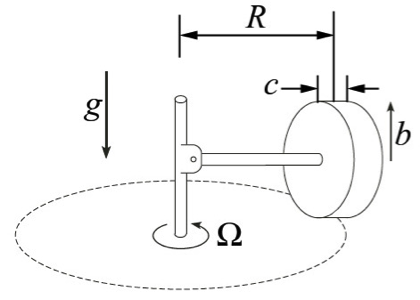
\includegraphics[scale=1.2]{Graphics/h8p9}
\end{center}

(a) How is the angular speed $\omega$ of the wheel about its axis related to the angular speed $\Omega$ about the shaft? Express your answer in terms of $\Omega$, $b$ and $R$.\\
(b) What is the horizontal component of the angular momentum vector about the point P in the figure above? Although we have not shown this, for this situation it is correct to compute the horizontal component of the angular momentum by completely ignoring the rotation of the mill wheel about the vertical axis, taking into account only the rotation of the mill wheel about its own axle. Express your answer in terms of $\Omega$, $M$, $b$ and $R$.\\
(c) What is the magnitude of the torque about the joint (about the point P in the figure above) due to the forces acting on the axle-wheel combination? Express your answer in terms of $N$, $R$, $M$, $g$.\\
(d) What is the value of $\Omega$ if the contact force between the stone and the ground $N = 2 M g$? Express your answer in terms of $b$ and $g$.''

Having read the section in the book (chapter 22) on exactly this problem, I feel like I'm cheating here! I will do what I can to derive everything I use, in order to ensure I understand it all, at least.

All right. The first part is rather easy, at least: the center of mass of the wheel must move with speed $v_{cm} = \omega b$ if there is no slip (this is a condition of pure roll). Meanwhile, the entire wheel is also rotating about the center axis with angular speed $\Omega$, which can be used to find $v_{cm} = \Omega R$ separately from the previous relationship.\\
We can then simply set the two equal and solve for $\omega$, since $\Omega$ is allowed in the answer:

\begin{align}
\omega b &= \Omega R\\
\omega   &= \frac{\Omega R}{b}
\end{align}

Next, the horizontal component of the angular momentum relative to point P. Given the hint in the problem, this is very easy. The angular momentum about the axle's axis due to the rotation (about the wheel's center of mass) is just $I_c \omega$, where we use $I_c = \frac{1}{2} M b^2$ for a solid disk of radius $b$ (not $R$ in this problem!):

\begin{equation}
L_P = I_c \omega = (\frac{1}{2} M b^2)\left(\frac{\Omega R}{b}\right) = \frac{\Omega R M b}{2}
\end{equation}

Part (c) is regarding the magnitude of the torque about the center axle (point P is not in the figure, but it is in the book; it is where the axle connects to the vertical bar, at the hinge).

Well, what forces could cause a torque? Gravity acting on the wheel certainly counts; the torque at P (see above) due to gravity acting on the wheel is $\tau_{P,gravity} = (\vec{R} \times \vec{g}) M = R M g$ (there is a 90 degree angle, so $\sin \theta = 1$), with the direction being into the page (causing rotation as shown for $\Omega$).\\
Next, there is the normal force $N = 2 M g$ causing a torque $\vec{R} \times \vec{N} = R N = 2 R M g$, with the direction being out of the page, opposing the previous torque.\\
If the axle is taken to be massless, there are no other forces that act such that they cause a torque relative to point P.

The net torque, or at least the magnitude of it, is just the torque due to the normal force minus the torque due to gravity:

\begin{equation}
|\tau_{P,net}| = R N - R M g
\end{equation}

We could write this in terms of $2 M g$ instead of $N$, but the grader really wants it in terms of $N$, according to the forum discussions. I submitted the above as the first attempt, and it was indeed accepted.

Finally, what is $\Omega$, in terms of only $b$ and $g$, at a time where $N = 2 M g$?\\
This is the precession frequency -- note how the system looks a lot like a gyroscope. (It's even as an example in the gyroscope section in the book.)

We learned in lecture that $\displaystyle \Omega = \frac{\tau}{L_{spin,cm}}$, but this only holds if $L_{spin,cm} \gg L_{orbital}$, which doesn't appear to be the case here. In the case of a typical gyroscope, the spin could be several thousand rpm ($200 \pi$ rad/s or more), while the orbits was closer to 5 per minute or even less.\\
Here, the two are much closer together.

We can solve this in (at least?) two ways. One is, in fact, to use the above equation:

\begin{align}
\Omega &= \frac{2 R M g - R M g}{\frac{1}{2} \Omega R M b}\\
\Omega^2 &= \frac{g}{\frac{1}{2} b}\\
\Omega &= \sqrt{\frac{2 g}{b}}
\end{align}

The second is to find the torque as $\displaystyle \frac{dL}{dt}$ (i.e. take the time derivative of $L$ above) and set that equal to the torque we found earlier. However, to do this properly, we need to consider the directions properly too. Check the book (chapter 22) for a proper derivation. The result is:

\begin{align}
\frac{dL}{dt} = \frac{\Omega^2 R M b}{2} &= R M g\\
                \Omega^2 b &= 2 g\\
                \Omega &= \sqrt{\frac{2 g}{b}}
\end{align}

The source of the extra $\Omega$ is tricky, since I have not written all this in terms of components and unit vectors. The source of it is due to the differentiation of the $\hat{r}$ unit vector:

\begin{equation}
\frac{d\hat{r}}{dt} = \frac{d\theta}{dt} \hat{\theta}
\end{equation}

where $\theta$ is the position along the circle, and $\hat{\theta}$ is the unit vector in the azimuthal direction (in cylindrical coordinates). $\Omega$ is just the time rate of change of this angle, by definition, so that $\displaystyle \Omega = \frac{d\theta}{dt}$. Therefore, in terms of vectors,

\begin{align}
\vec{L}_{spin,cm}             &= \frac{\Omega R M b}{2}(-\hat{r})\\
\frac{d\vec{L}_{spin,cm}}{dt} &= \frac{\Omega R M b}{2} \left(-\frac{d\hat{r}}{dt}\right) = \frac{\Omega R M b}{2} \left(-\Omega \hat{\theta}\right)
\end{align}

The magnitude is therefore multiplied by $\Omega$ in this differentiation. I apologize for the sloppiness here; again, check the book if you're looking for a rigorous treatment of this problem.

\section{Problem 10: Double drums rotating}

``A drum A of mass $M$ and radius $R$ is suspended from a drum B also of mass $M$ and radius $R$, which is free to rotate about its axis. The suspension is in the form of a massless metal tape wound around the outside of each drum, and free to unwind. Gravity is directed downwards. Both drums are initially at rest. Consider the drums to be uniform disks.

\begin{center}
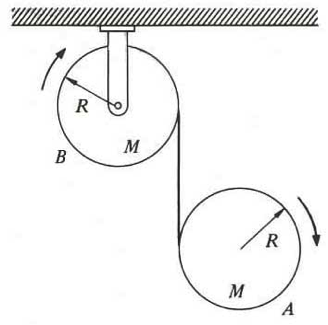
\includegraphics[scale=1.0]{Graphics/h8p10}
\end{center}

Find the initial acceleration of drum A, assuming that it moves straight down. Express your answer in terms of $M$, $R$ and acceleration due to gravity $g$ as needed.''

Because drum B (the one at the top) is free to rotate, this problem is not quite as easy as it might look to begin with. We must assume that it too rotates, and that the tape is unrolled from \emph{both} drums at the same time.

Okay then, let's see. First, let's consider the linear acceleration of drum A, which will certainly give us more than one unknown. Using downwards as the positive direction,

\begin{equation}
M a = M g - T
\end{equation}

The string (tape?) will unroll, which means we can also consider the angular acceleration, due to the torque provided by this tension. The torque relative to the center of drum A $\tau_A = I_c \alpha$, which is also simply $\vec{R} \times \vec{T}$, where $\vec{R}$ is the position vector from the center (since we take that as our origin for the torque) to the edge of drum A.

\begin{align}
R T &= \left(\frac{1}{2} M R^2\right) \alpha_A
\end{align}

Here is where we must be very careful. We can \emph{not} use $a = \alpha R$ here! That holds when the drum unrolls such that 100\% of the added length of tape comes from the drum -- but both drums are unrolling at the same time! In other words, we don't have pure roll in this situation. Instead, we must consider the torque and angular acceleration of drum B. Since both radius, mass and tension are all the same, we find

\begin{equation}
R T = \left(\frac{1}{2} M R^2\right) \alpha_B
\end{equation}

By comparing these two last equations, we don't even need to solve either so find $\alpha_A = \alpha_B$; everything except those variable names are the same in both equations.

Finally, we can consider the position (and change in position) considering how much tape is unrolled. Following the book's approach, an amount $R \Delta \theta_A$ is unrolled from the first drum in some time $\Delta t$, and the same thing except with a B index holds for drum B. The distance fallen for drum A is the sum of the two, i.e. the total amount of tape unwound. If we take the time derivative of these expressions, we get

\begin{equation}
\frac{dy}{dt} = R \frac{d\theta_A}{dt} + R \frac{d \theta_B}{dt}
\end{equation}

... and again:

\begin{equation}
\frac{d^2 y}{dt^2} = a = R(\alpha_A + \alpha_B)
\end{equation}

The values of $\alpha_A = \alpha_B$ in terms of the tension is

\begin{equation}
\frac{2 T}{M R} = \alpha_A = \alpha_B
\end{equation}

And using the first equation we found, $T = M(g - a)$, so

\begin{align}
\alpha_A &= \alpha_B = \frac{2}{M R} M(g - a)\\
\alpha_A &= \alpha_B = \frac{2}{R} (g - a)
\end{align}

So at this stage, we have two equations:

\begin{align}
\alpha_A = \alpha_B = \frac{2}{R} (g - a)\\
a = R(\alpha_A + \alpha_B)
\end{align}

Substitute the top one into the lower one:

\begin{align}
a &= 2 R(\frac{2}{R} (g - a))\\
a &= 4 g - 4 a\\
a &= \frac{4}{5} g
\end{align}

The acceleration is higher than the $\frac{2}{3} g$ we find if the top drum cannot spin, and we therefore assume pure roll.

\end{document}